\documentclass[twoside]{book}

% Packages required by doxygen
\usepackage{fixltx2e}
\usepackage{calc}
\usepackage{doxygen}
\usepackage[export]{adjustbox} % also loads graphicx
\usepackage{graphicx}
\usepackage[utf8]{inputenc}
\usepackage{makeidx}
\usepackage{multicol}
\usepackage{multirow}
\PassOptionsToPackage{warn}{textcomp}
\usepackage{textcomp}
\usepackage[nointegrals]{wasysym}
\usepackage[table]{xcolor}

% Font selection
\usepackage[T1]{fontenc}
\usepackage[scaled=.90]{helvet}
\usepackage{courier}
\usepackage{amssymb}
\usepackage{sectsty}
\renewcommand{\familydefault}{\sfdefault}
\allsectionsfont{%
  \fontseries{bc}\selectfont%
  \color{darkgray}%
}
\renewcommand{\DoxyLabelFont}{%
  \fontseries{bc}\selectfont%
  \color{darkgray}%
}
\newcommand{\+}{\discretionary{\mbox{\scriptsize$\hookleftarrow$}}{}{}}

% Page & text layout
\usepackage{geometry}
\geometry{%
  a4paper,%
  top=2.5cm,%
  bottom=2.5cm,%
  left=2.5cm,%
  right=2.5cm%
}
\tolerance=750
\hfuzz=15pt
\hbadness=750
\setlength{\emergencystretch}{15pt}
\setlength{\parindent}{0cm}
\setlength{\parskip}{3ex plus 2ex minus 2ex}
\makeatletter
\renewcommand{\paragraph}{%
  \@startsection{paragraph}{4}{0ex}{-1.0ex}{1.0ex}{%
    \normalfont\normalsize\bfseries\SS@parafont%
  }%
}
\renewcommand{\subparagraph}{%
  \@startsection{subparagraph}{5}{0ex}{-1.0ex}{1.0ex}{%
    \normalfont\normalsize\bfseries\SS@subparafont%
  }%
}
\makeatother

% Headers & footers
\usepackage{fancyhdr}
\pagestyle{fancyplain}
\fancyhead[LE]{\fancyplain{}{\bfseries\thepage}}
\fancyhead[CE]{\fancyplain{}{}}
\fancyhead[RE]{\fancyplain{}{\bfseries\leftmark}}
\fancyhead[LO]{\fancyplain{}{\bfseries\rightmark}}
\fancyhead[CO]{\fancyplain{}{}}
\fancyhead[RO]{\fancyplain{}{\bfseries\thepage}}
\fancyfoot[LE]{\fancyplain{}{}}
\fancyfoot[CE]{\fancyplain{}{}}
\fancyfoot[RE]{\fancyplain{}{\bfseries\scriptsize Generated by Doxygen }}
\fancyfoot[LO]{\fancyplain{}{\bfseries\scriptsize Generated by Doxygen }}
\fancyfoot[CO]{\fancyplain{}{}}
\fancyfoot[RO]{\fancyplain{}{}}
\renewcommand{\footrulewidth}{0.4pt}
\renewcommand{\chaptermark}[1]{%
  \markboth{#1}{}%
}
\renewcommand{\sectionmark}[1]{%
  \markright{\thesection\ #1}%
}

% Indices & bibliography
\usepackage{natbib}
\usepackage[titles]{tocloft}
\setcounter{tocdepth}{3}
\setcounter{secnumdepth}{5}
\makeindex

% Hyperlinks (required, but should be loaded last)
\usepackage{ifpdf}
\ifpdf
  \usepackage[pdftex,pagebackref=true]{hyperref}
\else
  \usepackage[ps2pdf,pagebackref=true]{hyperref}
\fi
\hypersetup{%
  colorlinks=true,%
  linkcolor=blue,%
  citecolor=blue,%
  unicode%
}

% Custom commands
\newcommand{\clearemptydoublepage}{%
  \newpage{\pagestyle{empty}\cleardoublepage}%
}

\usepackage{caption}
\captionsetup{labelsep=space,justification=centering,font={bf},singlelinecheck=off,skip=4pt,position=top}

%===== C O N T E N T S =====

\begin{document}

% Titlepage & ToC
\hypersetup{pageanchor=false,
             bookmarksnumbered=true,
             pdfencoding=unicode
            }
\pagenumbering{alph}
\begin{titlepage}
\vspace*{7cm}
\begin{center}%
{\Large Neural Network }\\
\vspace*{1cm}
{\large Generated by Doxygen 1.8.14}\\
\end{center}
\end{titlepage}
\clearemptydoublepage
\pagenumbering{roman}
\tableofcontents
\clearemptydoublepage
\pagenumbering{arabic}
\hypersetup{pageanchor=true}

%--- Begin generated contents ---
\chapter{Class Index}
\section{Class List}
Here are the classes, structs, unions and interfaces with brief descriptions\+:\begin{DoxyCompactList}
\item\contentsline{section}{\mbox{\hyperlink{classNetwork}{Network}} \\*\mbox{\hyperlink{classNetwork}{Network}} object the network object acts as a layer between the user and the input,hidden, and output layers }{\pageref{classNetwork}}{}
\end{DoxyCompactList}

\chapter{File Index}
\section{File List}
Here is a list of all documented files with brief descriptions\+:\begin{DoxyCompactList}
\item\contentsline{section}{Neural\+Network/includes/\mbox{\hyperlink{network_8h}{network.\+h}} \\*Header file for network object }{\pageref{network_8h}}{}
\item\contentsline{section}{Neural\+Network/src/\mbox{\hyperlink{nn_8cpp}{nn.\+cpp}} \\*File with int main }{\pageref{nn_8cpp}}{}
\item\contentsline{section}{Neural\+Network/src/libs/\mbox{\hyperlink{network_8cpp}{network.\+cpp}} \\*File containing definitions for network object }{\pageref{network_8cpp}}{}
\end{DoxyCompactList}

\chapter{Class Documentation}
\hypertarget{classNetwork}{}\section{Network Class Reference}
\label{classNetwork}\index{Network@{Network}}


\mbox{\hyperlink{classNetwork}{Network}} object the network object acts as a layer between the user and the input,hidden, and output layers.  




{\ttfamily \#include $<$network.\+h$>$}



Collaboration diagram for Network\+:\nopagebreak
\begin{figure}[H]
\begin{center}
\leavevmode
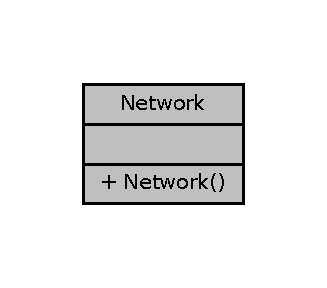
\includegraphics[width=157pt]{classNetwork__coll__graph}
\end{center}
\end{figure}
\subsection*{Public Member Functions}
\begin{DoxyCompactItemize}
\item 
\mbox{\Hypertarget{classNetwork_a3cc2fb4f8fa4d507077e8da85ce5a1c8}\label{classNetwork_a3cc2fb4f8fa4d507077e8da85ce5a1c8}} 
\mbox{\hyperlink{classNetwork_a3cc2fb4f8fa4d507077e8da85ce5a1c8}{Network}} ()
\begin{DoxyCompactList}\small\item\em Constructor that calls \+\_\+init\+\_\+network. \end{DoxyCompactList}\end{DoxyCompactItemize}


\subsection{Detailed Description}
\mbox{\hyperlink{classNetwork}{Network}} object the network object acts as a layer between the user and the input,hidden, and output layers. 

The documentation for this class was generated from the following files\+:\begin{DoxyCompactItemize}
\item 
Neural\+Network/includes/\mbox{\hyperlink{network_8h}{network.\+h}}\item 
Neural\+Network/src/libs/\mbox{\hyperlink{network_8cpp}{network.\+cpp}}\end{DoxyCompactItemize}

\chapter{File Documentation}
\hypertarget{network_8h}{}\section{Neural\+Network/includes/network.h File Reference}
\label{network_8h}\index{Neural\+Network/includes/network.\+h@{Neural\+Network/includes/network.\+h}}


header file for network object  


{\ttfamily \#include $<$vector$>$}\newline
{\ttfamily \#include $<$iostream$>$}\newline
Include dependency graph for network.\+h\+:
\nopagebreak
\begin{figure}[H]
\begin{center}
\leavevmode
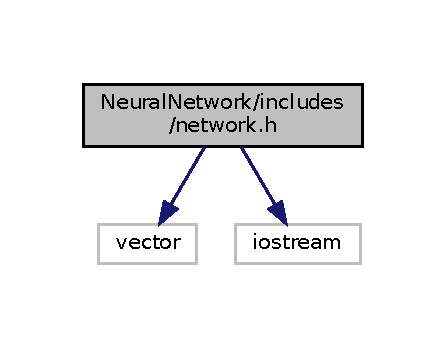
\includegraphics[width=214pt]{network_8h__incl}
\end{center}
\end{figure}
This graph shows which files directly or indirectly include this file\+:
\nopagebreak
\begin{figure}[H]
\begin{center}
\leavevmode
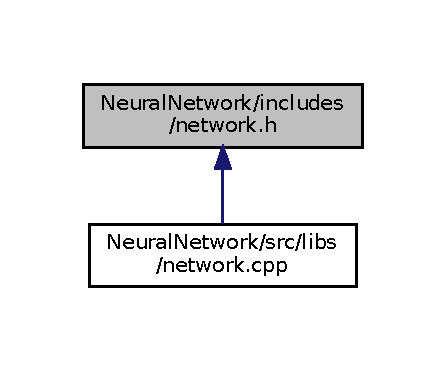
\includegraphics[width=214pt]{network_8h__dep__incl}
\end{center}
\end{figure}
\subsection*{Classes}
\begin{DoxyCompactItemize}
\item 
class \mbox{\hyperlink{classNetwork}{Network}}
\begin{DoxyCompactList}\small\item\em \mbox{\hyperlink{classNetwork}{Network}} object the network object acts as a layer between the user and the input,hidden, and output layers. \end{DoxyCompactList}\end{DoxyCompactItemize}


\subsection{Detailed Description}
header file for network object 

\begin{DoxyAuthor}{Author}
Minhyuk Park 
\end{DoxyAuthor}
\begin{DoxyDate}{Date}
8 Jun 2018 
\end{DoxyDate}

\hypertarget{network_8cpp}{}\section{Neural\+Network/src/libs/network.cpp File Reference}
\label{network_8cpp}\index{Neural\+Network/src/libs/network.\+cpp@{Neural\+Network/src/libs/network.\+cpp}}


File containing definitions for network object.  


{\ttfamily \#include \char`\"{}network.\+h\char`\"{}}\newline
Include dependency graph for network.\+cpp\+:
\nopagebreak
\begin{figure}[H]
\begin{center}
\leavevmode
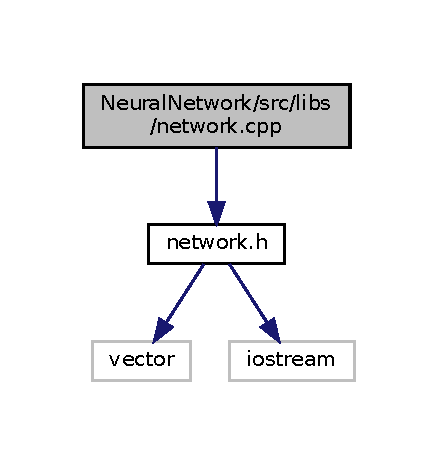
\includegraphics[width=210pt]{network_8cpp__incl}
\end{center}
\end{figure}


\subsection{Detailed Description}
File containing definitions for network object. 

\begin{DoxyAuthor}{Author}
Minhyuk Park 
\end{DoxyAuthor}
\begin{DoxyDate}{Date}
8 Jun 2018 
\end{DoxyDate}

\hypertarget{nn_8cpp}{}\section{Neural\+Network/src/nn.cpp File Reference}
\label{nn_8cpp}\index{Neural\+Network/src/nn.\+cpp@{Neural\+Network/src/nn.\+cpp}}


File with int main.  


{\ttfamily \#include $<$iostream$>$}\newline
Include dependency graph for nn.\+cpp\+:
\nopagebreak
\begin{figure}[H]
\begin{center}
\leavevmode
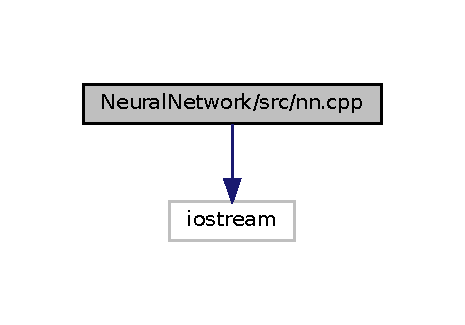
\includegraphics[width=223pt]{nn_8cpp__incl}
\end{center}
\end{figure}
\subsection*{Functions}
\begin{DoxyCompactItemize}
\item 
\mbox{\Hypertarget{nn_8cpp_ae66f6b31b5ad750f1fe042a706a4e3d4}\label{nn_8cpp_ae66f6b31b5ad750f1fe042a706a4e3d4}} 
int {\bfseries main} ()
\end{DoxyCompactItemize}


\subsection{Detailed Description}
File with int main. 

\begin{DoxyAuthor}{Author}
Minhyuk Park 
\end{DoxyAuthor}
\begin{DoxyDate}{Date}
8 Jun 2018 
\end{DoxyDate}

%--- End generated contents ---

% Index
\backmatter
\newpage
\phantomsection
\clearemptydoublepage
\addcontentsline{toc}{chapter}{Index}
\printindex

\end{document}
